%----------------------------------------------------------------------------------------
%	PACKAGES AND OTHER DOCUMENT CONFIGURATIONS
%----------------------------------------------------------------------------------------

\documentclass[10pt]{article}											% font size

\usepackage{myStyle}													% Use a custom style sheet: double column, police, text...
\usepackage{graphicx}													% to include images
\usepackage{float}														% to float figures
\usepackage{booktabs,makecell}											% for diagonal cells
\usepackage{hyperref}													% for hyperlinks
\usepackage{listings}													% for including files
%\usepackage[top=1in, bottom=1in, left=1.25in, right=1.25in]{geometry}	% set margins
\usepackage[top=0.75in, bottom=0.75in, left=0.75in, right=0.75in]{geometry}	% set margins
\usepackage[utf8]{inputenc}												% for unicode input characters
\usepackage{helvet}														% use helvetica per default
\usepackage[T1]{fontenc}
\usepackage[english]{babel}
\usepackage{multicol}													% To make the document with many columns

\setlength{\columnsep}{1cm}
\renewcommand{\familydefault}{\sfdefault}								% use sans serif per default

\lstset
{
  basicstyle=\scriptsize\sffamily,%
  commentstyle=\footnotesize\ttfamily,%
  frameround=trBL,
  frame=single,
  breaklines=true,
  showstringspaces=false,
  numbers=left,
  numberstyle=\tiny,
  numbersep=10pt,
  keywordstyle=\bf
}


%----------------------------------------------------------------------------------------
%	TITLE SECTION 
%----------------------------------------------------------------------------------------

\makeatletter
\makeatother
\renewcommand{\familydefault}{\sfdefault} % use sans serif per default
\makeatother

\begin{document}

\title{Impact of memory allocation on the performance of a delegation synchronization algorithm}
\author{Written by Riyane SID-LAKHDAR (M1 MoSIG)\\
Supervised by Thomas ROPARS (LIG, team ERODS)}
\maketitle




%----------------------------------------------------------------------------------------
%	ABSTRACT
%----------------------------------------------------------------------------------------


%\tableofcontents

\begin{abstract}
****************************** TODO\\
	- Context\\
	- problems\\
	- Results\\
	- Conclusion\\

***** Trouver des synonimes a performance issue: downgrading/drop/reduction/decline/deterioration/ 
********************* End TODO
\end{abstract}

****************************** TODO\\
	- Modifier imperativement les tittres (AHHHHHHH)\\
    - Verifier les temps et les formes des tittres (passives/actives)\\
*********************** End TODO


%----------------------------------------------------------------------------------------
%	INTRODUCTION
%----------------------------------------------------------------------------------------
\section{Introduction}
With the rise of many-core processors, concurrent programs have increased the efficiency of existing algorithms by simply splitting their tasks over different executors at the same time.   However, due to hardware and software issues, parallelizing the execution of a task using \textit{N} cores does not mean dividing its execution time by \textit{N}.\\

Among the things that can limit the efficiency of concurrent algorithms, memory allocation is one that is often disregarded but that can still deeply affect the performance. The main problem when dealing with a large number of threads,  that frequently allocate and free memory, is that the memory allocation system may receive requests from different threads at the same time.   As the memory allocation system answers the requests sequentially, it becomes the performance bottleneck of multithreading.\\

Another issue for multithreaded applications is the need to synchronization for concurrent memory access.   In this context, \textit{delegation} is an example of contributions to efficiently implement mutual exclusion on shared objects.   However, existing evaluations of \textit{delegation} algorithms are obtained using unrealistic allocators \footnote{Allocators that outperform the time efficiency of general-purpose allocators by using a relatively large and thread local dynamic memory.   Hence, such an allocator can not be used as a general purpose one.}.   Hence our main aim is to study how delegation algorithms would perform when used with state-of-the-art general-purpose allocators.

Different strategies have been proposed to improve the efficiency of the dynamic memory management.   Thus, in the present work, we present, first of all, a description of the main allocators for multithreaded systems.   We show how the complexity and the heterogeneity of this implementations could dramatically influence the performance of any algorithm for shared memory management.\\
Second, in order to asses the efficiency of these strategies, we present a custom environment and a set of realistic tests to stress allocators that implement them.   Thanks to this testing platform, we are able to compare these strategies under stringent conditions.\\
Finally, our third contribution is to present an evaluation of two delegation algorithms (see section \ref{delegationSynchronizationAlgo_description}) using the allocation strategy that best fits our workbench.\\

************\\
Results\\
************\\



%----------------------------------------------------------------------------------------
%	CONTEXT AND MOTIVATION
%----------------------------------------------------------------------------------------

\section{Context and motivation}
Any application that tries to manage dynamic memory faces a set of issues that impact its performance.   In this section, we highlight these issues.   We also explain how the complexity and the heterogeneity of these challenges motivate the need beneath the comparison of allocators: an inefficient allocator may dramatically influence the tests of our delegation target algorithms \cite{delegationCS_roparsPetrovic}.


%----------------------------------------------------------------------------------------

\subsection{Complex processor architecture}
Let us consider a \textit{Non Uniform Memory Access (NUMA)} processor (see figure \ref{globalNumaArchitecture.png}).   To maintain a set of data coherent and up-to-date over such an architecture, an important time and space overhead is required.   Indeed, this architecture represents a complex structure with several levels of caches which need to stay coherent at any time.   And these properties have to hold despite the different cores (or even different processing units on the same core for \textit{hyper-threaded processors}) which may access the caches asynchronously.\\

	\begin{figure}
		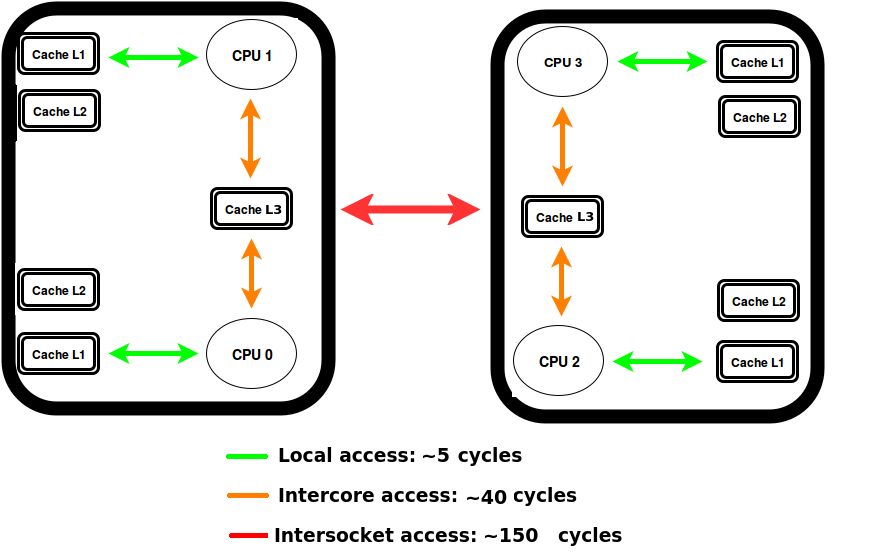
\includegraphics[width=1.0\linewidth]{charts/numaNode.png}
		\caption{Simplified NUMA model (only $\frac{3}{8}$ memory access types)}
        \label{globalNumaArchitecture.png}
	\end{figure}

The hardware architectures (NUMA) that we consider are made of independent units over the same processor.   Thus, any interaction between two independent components involves network communication protocols.  Hence a non negligible over-cost.\\
When a thread tries to reach an address kept by its current L1 cache, the access may be done in a relatively short time (about 2 CPU cycles).   However, this value may dramatically increase when the address is kept by a foreign core:  up to 200 CPU cycles when the core is on the same NUMA node (L3 cache) and 1500 CPU cycles when the core is on a foreign node (socket communication).


%----------------------------------------------------------------------------------------

\subsection{False sharing memory blowup and heavy kernel processes}
The allocation and the liberation of dynamic memory is unpredictable \footnote{However we can detect memory access patterns, all we can do is to have a probabilistic prevision model} and asynchronous.   Thus, after a period of time, any set of dynamically-used memory may become fragmented:   blocks of free and used memory are relatively small and highly interleaved.\\
Dealing with a fragmented dynamic memory may impact the allocation performance:   when the user requires a given block of memory, the allocator may have no free chunk of memory large enough to satisfy the request, while the total free memory may still be enough.   Depending on the allocator implementation, the request may remain unsatisfied, or the process heap may be dynamically expanded.   But in all cases a non negligible delay is appended to the allocation time.   This performance deterioration is known as \textbf{\textit{memory blowup}}.\\

	\begin{figure}
				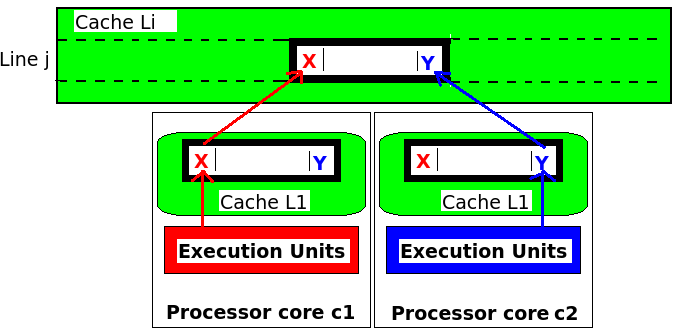
\includegraphics[width=1.0\linewidth]{charts/falseSharing.png}
		\caption{False sharing representation}
		\label{falseSharing.png}
	\end{figure}

Another performance drop, known as \textbf{\textit{false sharing}} may appear at access time.   Let us consider two separated objects accessed by two different threads running concurrently on two different cores.   Let us also suppose that the two objects are stored in the same cache line (see figure \ref{falseSharing.png}).   As these objects have different address ranges, they could safely be accessed simultaneously.   However, as the accesses granularity in the cache is a cache line (typically 64 Bytes), the cache controller will execute these accesses sequentially, increasing thus the total access time.\\

Finally, the paged memory is a resource shared by independent processes running on separate cores within one or multi-processors.   Managing this memory must be done at kernel level through an interaction between all these hardware and software components.   Thus, any memory allocator is subjected to the use of a set of heavy process, often involving context switches.


%----------------------------------------------------------------------------------------

\subsection{Testing a new algorithmic approach: Delegation for shared memory access}
Our paper follows the work of \textit{D. Petrovic}, \textit{T. Ropars} and \textit{A. Scipher}\cite{delegationCS_roparsPetrovic}.   In this former paper, an algorithm, based on the \textbf{\textit{delegation approach}} is described in order to access concurrently a shared object (see section \ref{delegationSynchronizationAlgo_description}).   This algorithm is experimentally shown as achieving "1.4x (resp. 2x) higher throughput compared to the most efficient state-of-the-art delegation solution" \cite{delegationCS_roparsPetrovic}.\\

One limitation of their study is that the experimental tests of the developed algorithms have been lead using a \textit{custom allocator}, built in order to allocate and free memory in short and roughly constant time (ideal allocator).   But which could not hold at scale\footnote{The principle of this allocator is to pin to each thread a block of memory at creation time.   The dynamic memory management is optimized by always allocating from this block.   No address of this block is freed until the thread destruction.}.

Regarding the wild scope and the complexity of the challenges associated with dynamic memory allocation (previous sections), one can wonder how the use of a \textit{general-purpose allocator} could affect the performance and behavior of the synchronization algorithms \cite{delegationCS_roparsPetrovic}.   To answer this question, we need to identify the most suitable general-purpose allocator for our workload.






%----------------------------------------------------------------------------------------
%	STATE OF THE ART
%----------------------------------------------------------------------------------------

\section{State of the art}
As many-core machines have become wildly used, different memory allocators \cite{glibc_robertson,hoard_berger,scalloc_aigner,supermalloc_kuszmaul,jemalloc_evans,tcmalloc_ghemawat} have been proposed to try to fit the needs of this programming paradigm.   Each of these implementations has either proposed some new memory-allocation strategies or has improved an existing one.   In this section, we give an overview of some of these strategies.  We highlight their hardware and software advantages.  Finally,  we link them to some existing implementations.


%----------------------------------------------------------------------------------------

\subsection{Delegate memory allocation to user space program}
Among the set of functions that an operating system (OS) proposes to user program, the ones that trigger a system call are probably the costlier in terms of time (only considering the non blocking instructions).   They imply a context switch before each execution, increasing the execution time of the task.\\

In the \textit{Linux OS} C standard library \textbf{\textit{glibc}}\cite{glibc_robertson}, memory allocation function regularly re-sizes a process heap at runtime.  Thus, allocation functions may trigger system calls\footnote{Call to the kernel functions \textit{brk}, \textit{sbrk} and \textit{mmap}}.   To decrease to almost zero the number of these system calls, all the memory allocators that we will consider use the same strategy: a large chunk of memory is initially allocated to all user programs.   Allocation is then done at user level by simply splitting this initial chunk of memory.\\

Using this method dramatically decreases the number of system calls.  Yet, this number is not always null.  Indeed, when the initially allocated-memory is exceeded, user allocators may trigger a system call to seek the OS for a new chunk of memory (as used in \textit{Hoard}\cite{hoard_berger} or in \textit{SuperMalloc}\cite{supermalloc_kuszmaul}) or to answer each new allocation request made by the user (as used in \textit{Scalloc}\cite{scalloc_aigner}).


%----------------------------------------------------------------------------------------

\subsection{Core locality allocation}
Within \textit{UNIX} processes, dynamic memory (heap of the process) is a resource shared by many threads.   Thus, to ensure the consistency of the resource, synchronization is required between threads that try to access it, which obviously introduces a time override.\\

To decrease this synchronization override, \textbf{\textit{Hoard}}\cite{hoard_berger}, which is one of the first thread-scalable allocators, has introduced the idea of core locality:  each processor core is mapped to a unique buffer. Threads running on this core are the only one authorized to allocate memory in this buffer. Hence, allocation requires no synchronization between threads from different cores.   This idea has been further improved by \textbf{\textit{Scalloc}}\cite{scalloc_aigner} by adapting the data structure used for a buffer (see section \ref{virtualSpanDefinition})\\

One of the main advantages of the core local buffer is on the probability that a thread triggers a page fault.   Indeed, a buffer is allocated as a block of contiguous addresses.   All the threads running on a given core allocate memory within the same address range (addresses of the buffer).   Thus the probability to trigger a page fault is low, even after a context switch.


%----------------------------------------------------------------------------------------

\subsection{Dealing with the shared pool contention}
To feed each core-mapped buffer, an allocator may reuse a freed memory previously belonging to the same buffer (with no synchronization over-cost).   It also needs a structure supplying an empty buffer request (see figure \ref{globalArchitecture.png}).\\
This structure is made of one stack per core.  Hence, it may be safely accessed by all the core-local buffers simultaneously and without any synchronization.\\

\begin{figure}[H]
    \centering
    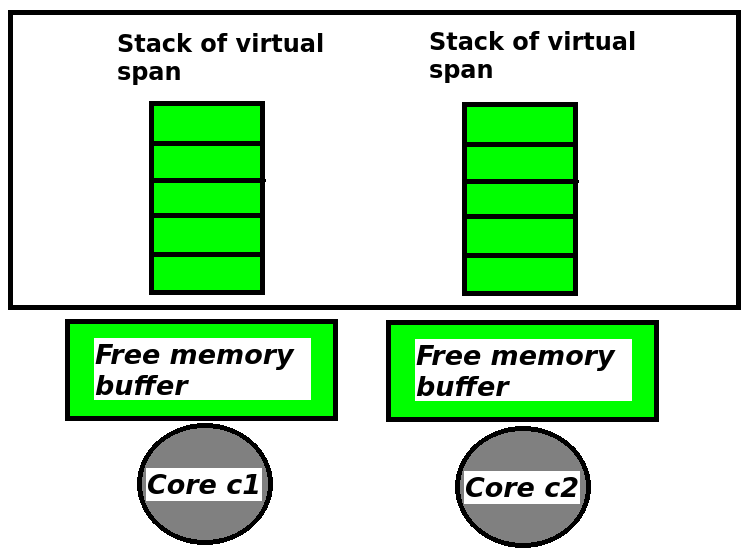
\includegraphics[width=0.4\textwidth]{charts/globalArchitecture.png}
    \caption[Caption for FN]{Free memory pool: shared by all the cores. TLAB: Thread Local Allocation Buffer}
    \label{globalArchitecture.png}
\end{figure}

One important efficiency factor of this shared structure is the number of requests it makes to the OS kernel to get more free memory.   To reduce this number, the policy introduced by \textbf{\textit{supermalloc}}\cite{supermalloc_kuszmaul} is to maintain the fill rate of all the core-mapped stacks roughly equal.   The OS kernel requests are only made once the average level of the stacks reaches a given threshold value.\\
Using such a policy, a core-mapped stack that runs out of memory will very likely be filled from another stack.  This contention on the core-mapped stacks has been lightened by \textbf{\textit{scalloc}}\cite{scalloc_aigner} through the usage of a \textit{Treiber stack}\footnote{The Treriber stack algorithm uses hardware atomic operations instead of locks in order to access concurrently the stack}.\\

These strategies have made it possible to remove almost all synchronization for allocation operations, making them having a roughly constant number of micro instructions.   However, a chunk of memory allocated by a given thread may be freed by a different one.   Thus, to avoid a synchronization over-cost for the \textit{free} operation, \textbf{\textit{scalloc}}\cite{scalloc_aigner} does not return a freed memory to the shared pool.  It places it instead into the buffer of the thread which runs the \textit{free} function.


%----------------------------------------------------------------------------------------

\subsection{Virtual span} \label{virtualSpanDefinition}
So far, we have considered improving the efficiency of memory management by adapting the \textit{allocation} and \textit{free} operations.   We can add further improvements by reducing the access time of a given address.

Within \textbf{\textit{scalloc}}\cite{scalloc_aigner} and \textbf{\textit{jemalloc}}\cite{jemalloc_evans}, the free memory has been organized using the principle of so-called \emph{virtual span}\footnote{Also called \emph{superblock} (resp \emph{superpage}) for \emph{Hoard}\cite{hoard_berger} (resp \emph{jemalloc}\cite{jemalloc_evans}) implementation.}.   This structure consists of a fixed-size block of contiguous addresses.   Nine different size classes exist, each of them is a multiple of 4KB (the size of a system page).   An allocation results in the use of one independent span, no matter the size required by the user. 
The payload of the object is stored into the span.   Additionally, some extra memory is used for alignment and uniformity purposes.\\

This architecture has been designed in order to face three major issues, which have been described earlier: \emph{space locality}, \emph{fragmentation} and \emph{complex data structures}.   We discuss next the available solutions\footnote{\emph{False sharing} is also dramatically reduced thanks to the virtual span.   An experimental evaluation of this improvement is available in \cite{scalloc_aigner}}.


%----------------------------------------------------------------------------------------

\subsubsection{Space locality}
The operating systems that we are considering implement \emph{virtual paging}.   Thus, a major concern for time efficiency is that memory addresses, which are more likely to be used together, may belong to the same page.   This property reduces the number of page faults, which is the major time consuming factor.\\
As a virtual span is a set of contiguous addresses, it increases the probability that two addresses of the same object (allocated by the same call to the “allocation” function) belong to the same page.


%----------------------------------------------------------------------------------------

\subsubsection{Fragmentation and complex data structures}
Storing exclusively a few number of size-range objects has an obvious interest for avoiding fragmentation.   On the other hand, as we treat uniformly large and small objects, an important extra memory may be required for small objects.   However, thanks to the paging system, this unused memory is swapped out of the live memory (RAM) and will never trigger a page fault (never called by the user).   Thus, the pagination system limits the time and space impact of the extra memory used by a span.


%----------------------------------------------------------------------------------------
%\subsection{Face memory blowup}
%\subsection{garbage collection}
%**********TODO**************








%----------------------------------------------------------------------------------------
%	MATERIAL AND METHODS
%----------------------------------------------------------------------------------------

\section{Material and methods}
\subsection{Custom delegation algorithms for synchronization}\label{delegationSynchronizationAlgo_description}
The algorithms we want to evaluate\cite{delegationCS_roparsPetrovic,combinerSyhcronization_darko} represent a way to access a critical section based on the \emph{delegation} principle: given a critical section CS, each thread that tries to access it will send a request to a dedicated centralized thread (server).   The server will answer the requests sequentially, by being the only one to access (and realize) the CS.\\


%----------------------------------------------------------------------------------------

\subsubsection{The \emph{combiner} algorithm}
In this algorithm, the server thread is not a specific dedicated one.   Indeed, when different client threads try to access a critical section CS, one of these threads is elected to execute its own CS as well as the one of a certain number of other threads.


%----------------------------------------------------------------------------------------

\subsubsection{\emph{Back-off with local spinning} and and \emph{Streaming store}}
This second algorithm implements two main improvements to the delegation method.

First, let us consider a client thread that has written a request to the server, and which spins on a specific memory address M, waiting for the answer.   The first improvement consists in adjusting this spinning rate to the \textit{prefetcher} rate, in order to delay the first read access of the client.   Thus, we increase the probability that the server realizes the CS between the client's write and the first client's read.   As the server holds a \emph{read write} access on M during this period, it may write the answer without updating the client's cache:  Thus it reduces the overhead due to a remote memory reference.

The second improvement consists in using a non temporal memory access (streaming) for the communication between the clients and the server.   Therefore, the server avoids waiting for the client acknowledgment, increasing the global throughput of satisfied requests.


%----------------------------------------------------------------------------------------

\subsection{Experimental setup and purpose}
In order to test the impact of different hardware NUMA architectures on the considered allocators, we have designed a testing platform which may adapt itself to a large number of processors and kernels.   This distributed platform has been launched on the test-bed \textit{Grid5000}.\\
The results that are presented in this paper have been obtained on two x86 machines.   The first one is an \textit{Dell Poweredge C6220} consisting of two 10-core \textit{Intel Xeon E5-2660v2} (2.2GHz) chips.   The second one is an \textit{HP Proliant DL165 G7} consisting of two 12-core \textit{AMD Opteron 6164 HE} (1.7 GHz) chips.
None of the considered machines perform \textit{Surface-mount technology} (hyper threading).\\
*********TODO\\
	- OS and kernel version
    - List of kernel policies: numactl (home node linked to a node or set of nodes: membind, interleave, first touch) transactional memory (allow atomic memory read and write)\\
**********End TODO\\
All the programs that implement the CS algorithms and the shared data structures have been implemented in C language.   They have been compiled using \textit{gcc 4.4.7} over all the considered machines.  The option O3 (maximum optimization level) has been used for all the compilation process.\\

This experimental setup has been used as an environment to host the programs implementing the two previous delegation algorithms.   It has also been used to host all the previously cited allocators: \emph{glibc} 3.74, \emph{Hoard} v2.2.1, \emph{scalloc} (released in August 2015), \emph{Supermalloc} (released in June 2015), \emph{gperftool-tcmalloc} v 3.2.1 and \emph{jemalloc} 4.2.1. 


%----------------------------------------------------------------------------------------

\subsection{Testing environment and rules}
The algorithms and implementations that we consider are designed to be used within general-purpose applications.   However, to test and compare them fairly, we have designed a specific environment which eliminates all extra costs which are outside the scope of our current study:
\begin{itemize}
	\item Each application we consider will use less threads than the number of cores available on the machine.   This constraint helps in lightening the waiting time due to scheduling.
	\item Each thread always run on the same core for the whole experiment.   This constraint is imposed to avoid the overhead linked to the synchronization of the same thread on different cores.   It also eliminates the cost of reaching an address owned by a cache within another core.   Finally, pining each thread to a respective core eliminates OS scheduler inference on the performance charts.
\end{itemize}







%----------------------------------------------------------------------------------------
%	RESULTS
%----------------------------------------------------------------------------------------
\section{Results}
In this section we use the \textit{throughput} and the \textit{global processor fairness} as metrics for our comparative study.   Other metrics such as the \textit{latency} or the \textit{inter-core fairness}, have been considered.   However, they have been omitted on purpose in this paper as they did not add any significant interest.\\


%----------------------------------------------------------------------------------------

\subsection{Choosing the most efficient memory allocator}
First, we evaluate the impact of the memory allocator on the throughput of an application implemented as a set of concurrent threads that loop on the access to a shared queue.  The shared queue is implemented using the \emph{combiner algorithm}.   Each appended (respectively removed) element is allocated (freed) dynamically.   The figure \ref{allocatorComparison.png} shows the throughput of this application when different allocators are used.

\begin{figure*}[!htb]\centering
	\begin{minipage}{0.35\textwidth}
		\frame{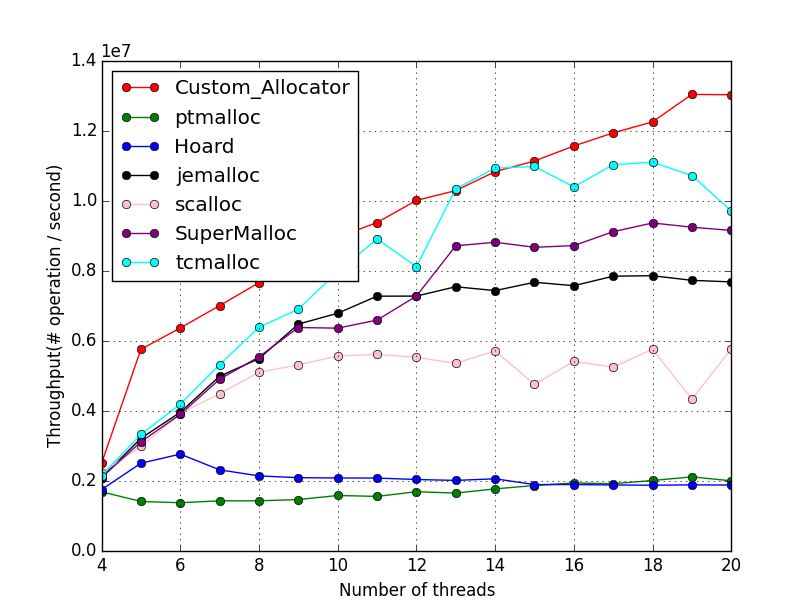
\includegraphics[width=\linewidth]{charts_allocator/20-Intel_Xeon_E5_2620-noOption-0-cc-msqueue.png}}
        \caption{Intel Xeon E5 2620}
	\end{minipage}
	\begin{minipage}{0.35\textwidth}
		\frame{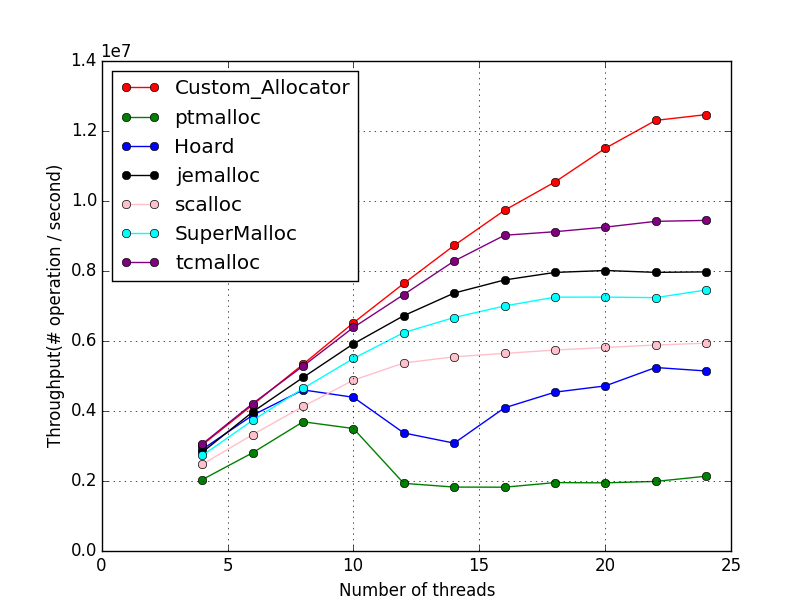
\includegraphics[width=\linewidth]{charts_allocator/24-AMD_Opteron_6164_HE-noOption-0-cc-msqueue.png}}
        \caption{AMD Opteron 6164 HE}
	\end{minipage}
	\caption{Impact of the memory allocator on the performance of multithreaded application}
	\label{allocatorComparison.png}
\end{figure*}

We can notice on this figures three main group of allocators, gathered according to their performances:\\
In a hand, the \textit{Unrealistic} (respectively \textit{glibc}) allocator which, as expected, outperforms (underperforms) all the others from 20\% up to 530\%.   In an other hand, the general purpose allocator may be sorted according to them implemented strategies:
\begin{itemize}
	\item \textit{Hoard}, which only implements the core local buffer is the less efficient one.   It has also the less stable behavior due to the non reuse of the freed memory: after a given period of time, the core local buffers get empty, and a system call (sequential) is required to feed them.   The more concurrent threads are running, the more this phenomena is important.  Which explains the dramatic decrease in the \textit{Hoards}'s curve after 10 threads.
	\item \textit{SuperMalloc, scalloc} and \textit{jemalloc} may be considered as equivalent.   The difference that we could notice on them curves are due to the management of the released memory.   Indeed, \textit{jemalloc} puts it into the shared pool while \textit{SuperMalloc} and \textit{scalloc} put it into the core local buffer, witch requires a synchronization with the next threads that allocate memory (within the core local buffer).
	\item \textit{tcmalloc} **********TODO *******
\end{itemize}


%----------------------------------------------------------------------------------------

\subsection{Custom delegation algorithm performance using a real allocator}
Thanks to the previous experimental results, we can definitely choose \textit{tcmalloc} as an allocator for the benchmark study of the considered delegation algorithms.\\
Using this allocator, we present on the figure \ref{delegationAlgorithmComparison.png} the performance comparison of a shared queue implemented using each of the considered delegation algorithms.

\begin{figure*}[!htb]\centering
	\begin{minipage}{0.35\textwidth}
		\frame{\includegraphics[width=\linewidth]{charts_allocator/20-Intel_Xeon_E5_2620-noOption-0-cc-msqueue+350-mp-msqueue-2-tcmalloc.png}}
        \caption{Intel Xeon E5 2620}
	\end{minipage}
	\begin{minipage}{0.35\textwidth}
		\frame{\includegraphics[width=\linewidth]{charts_allocator/24-AMD_Opteron_6164_HE-noOption-0-cc-msqueue+400-mp-msqueue-1-tcmalloc.png}}
		\caption{AMD Opteron 6164 HE}
	\end{minipage}
	\caption{Delegation algorithm comparison using the tcmalloc allocator. cc-msqueue:  shared queue implemented using the combiner algorithm.   mp-msqueue-2: shared queue implemented using the backoff/streaming delegation algorithm}
	\label{delegationAlgorithmComparison.png}
\end{figure*}




%----------------------------------------------------------------------------------------
%	CONCLUSION / DISCUSSION
%----------------------------------------------------------------------------------------
\section{Conclusion / Discussion}
From the above experimental results, three noteworthy results may come out.\\
First of all, the figure \ref{allocatorComparison.png} shows the highly significant difference between the unrealistic allocator used in the former test of the delegation algorithm, and the general purpose allocators.   It also shows how stable is the behaviour of this unrealistic allocator compared to the others.   This confirms the need to the current benchmarking study in order to confirm or infirm any performance property of the custom delegation algorithms.\\

Second, our method has confirmed the results obtained by \emph{D. Petrovic et al} \cite{delegationCS_roparsPetrovic} on the considered Intel architecture.   The optimized delegation algorithm allows in this specific condition to reach a higher throughput than the combiner algorithm (about 10\%).  And this result holds using both \textit{unrealistic} and \textit{tcmalloc} allocators.\\
However, our experimental results infirm the claim of \emph{D. Petrovic et al} \cite{delegationCS_roparsPetrovic} on the considered AMD architecture.   Indeed, within this specific conditions, the combiner algorithm reaches a higher throughput.   ********TODO *******\\

Finally, it is interesting to notice that during our experiments, we have reached a maximum throughput of $1.1 10^7$ (respectively $9.7 10^6$) on the considered Intel (respectively AMD) architecture using only 20 (respectively 24) hardware threads.   In the same time, the experimental results of \emph{D. Petrovic et al} has barely reached the same threshold throughput using ******TODDO *********** (respectively ***********TODO ******** ) hardware threads.   This hardware capacity difference highlight an important aspect of such a study:   all the conclusions that come out of our experimental results are highly dependent from the two considered hardware platforms and kernel policies.   Despite the remarkable similitude between our hardware platform and the one used by \emph{D. Petrovic et al}, the comparison and the link between the two studies is intrinsically dependent from this hardware difference.



%----------------------------------------------------------------------------------------
%	REFERENCES
%----------------------------------------------------------------------------------------
\section{Literature cited}

\nocite{*}
\small{\bibliographystyle{unsrt}
\bibliography{bibliography.bib}\vspace{0.75in}}





%----------------------------------------------------------------------------------------
%	ACKNOWLEDGMENT
%----------------------------------------------------------------------------------------
\section{Acknowledgment}


\end{document}